\begin{titlepage}
    \begin{center}

        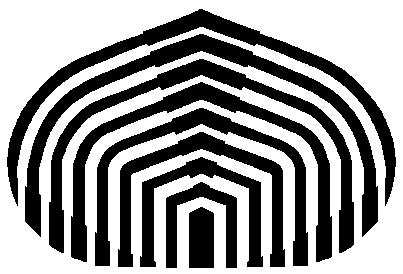
\includegraphics[width=1.2in]{partes/usb.png} \\
        \textsc {\large UNIVERSIDAD SIMÓN BOLÍVAR} \\
        \textsc{DECANATO DE ESTUDIOS PROFESIONALES\\
        COORDINACIÓN DE INGENIERÍA DE COMPUTACIÓN}\\ 
        \vfill
        \textbf{IMPLEMENTACIÓN DE UN ALGORITMO DE EVITACIÓN DE OBSTÁCULOS PARA DRONES AUTÓNOMOS} \\
        \vfill
        PROYECTO DE GRADO \\
        PRESENTADO POR: \\
        Joao Bose Pinto Diaz, 17-10490

    \end{center}
% El resumen debe ser de una sola página
\addtotoc{Resumen}
\vspace{-0.25cm}
\abstract
{   
\addtocontents{toc}{\vspace{1em}}

En el ámbito de la tecnología de drones, la seguridad de las operaciones es un elemento crucial para lograr una integración exitosa en diversas aplicaciones, desde la entrega de paquetes hasta la inspección de infraestructuras críticas. Este trabajo se enfocó en la implementación de un algoritmo de evasión de obstáculos para un dron comercial de cuatro rotores, utilizando el método basado en redes neuronales convolucionales propuesto por Loquercio et al. (2021) \cite{Loquercio2021}. Este método recibe como entrada un mapa de profundidad, el estado cinemático del dron y una dirección objetivo, y predice tres posibles trayectorias libres de colisión para el próximo segundo de vuelo. Para adaptar el método a las especificaciones de seguridad de la plataforma física, en particular, reducir la rapidez de ejecución, se realizó un refinamiento fino de los pesos del modelo utilizando una base de datos generada en el mismo entorno de simulación utilizado en el trabajo original, pero con una rapidez de 1 m/s en lugar de 7 m/s. La capacidad del algoritmo implementado para esquivar obstáculos se evaluó tanto en entornos de simulación como en entornos reales. Los resultados revelaron una preferencia del algoritmo por esquivar obstáculos por el flanco izquierdo, lo que produce colisiones en situaciones donde esta preferencia no es viable. Esta tendencia se atribuyó a un desbalance en la consideración de trayectorias sin colisión durante la generación de la base de datos. En este contexto, se propusieron posibles soluciones para mejorar el rendimiento y la capacidad de generalización del algoritmo en futuros trabajos.

}

% Las palabras clave son generalmente los nombres de áreas de investigación a
% los cuales está asociado el trabajo. Generalmente son tres o cuatro.
\noindent \begin{small} \textbf{Palabras clave}: Evasión de obstáculos, Vehículos aéreos no tripulados, Redes neuronales convolucionales. \end{small}

% Iniciar nueva página luego del resumen
\setstretch{1.2}

\end{titlepage}
